\subsection{Redundancia y diversidad en sistemas ferroviarios}

	La redundancia en sistemas críticos se define mediante la abreviatura NooM (N de M, del inglés, N out of M). Donde M representa la cantidad de módulos de medición/decisión que posee el sistema y N la cantidad de módulos que deben funcionar correctamente para que el sistema opere normalmente \cite{Paper_12,Paper_41,Paper_47,Paper_78,Paper_80,Paper_82,Paper_84}. En la Figura \ref{fig:redundancia} se puede apreciar un sistema con redundancia 2oo3, en el cual se tendrá una salida correcta siempre que se tenga a lo sumo un fallo por vez, no acumulativo. El sistema determina, mediante votación, la respuesta correcta a presentar como salida.
	
	\begin{figure}[H]
		\centering
		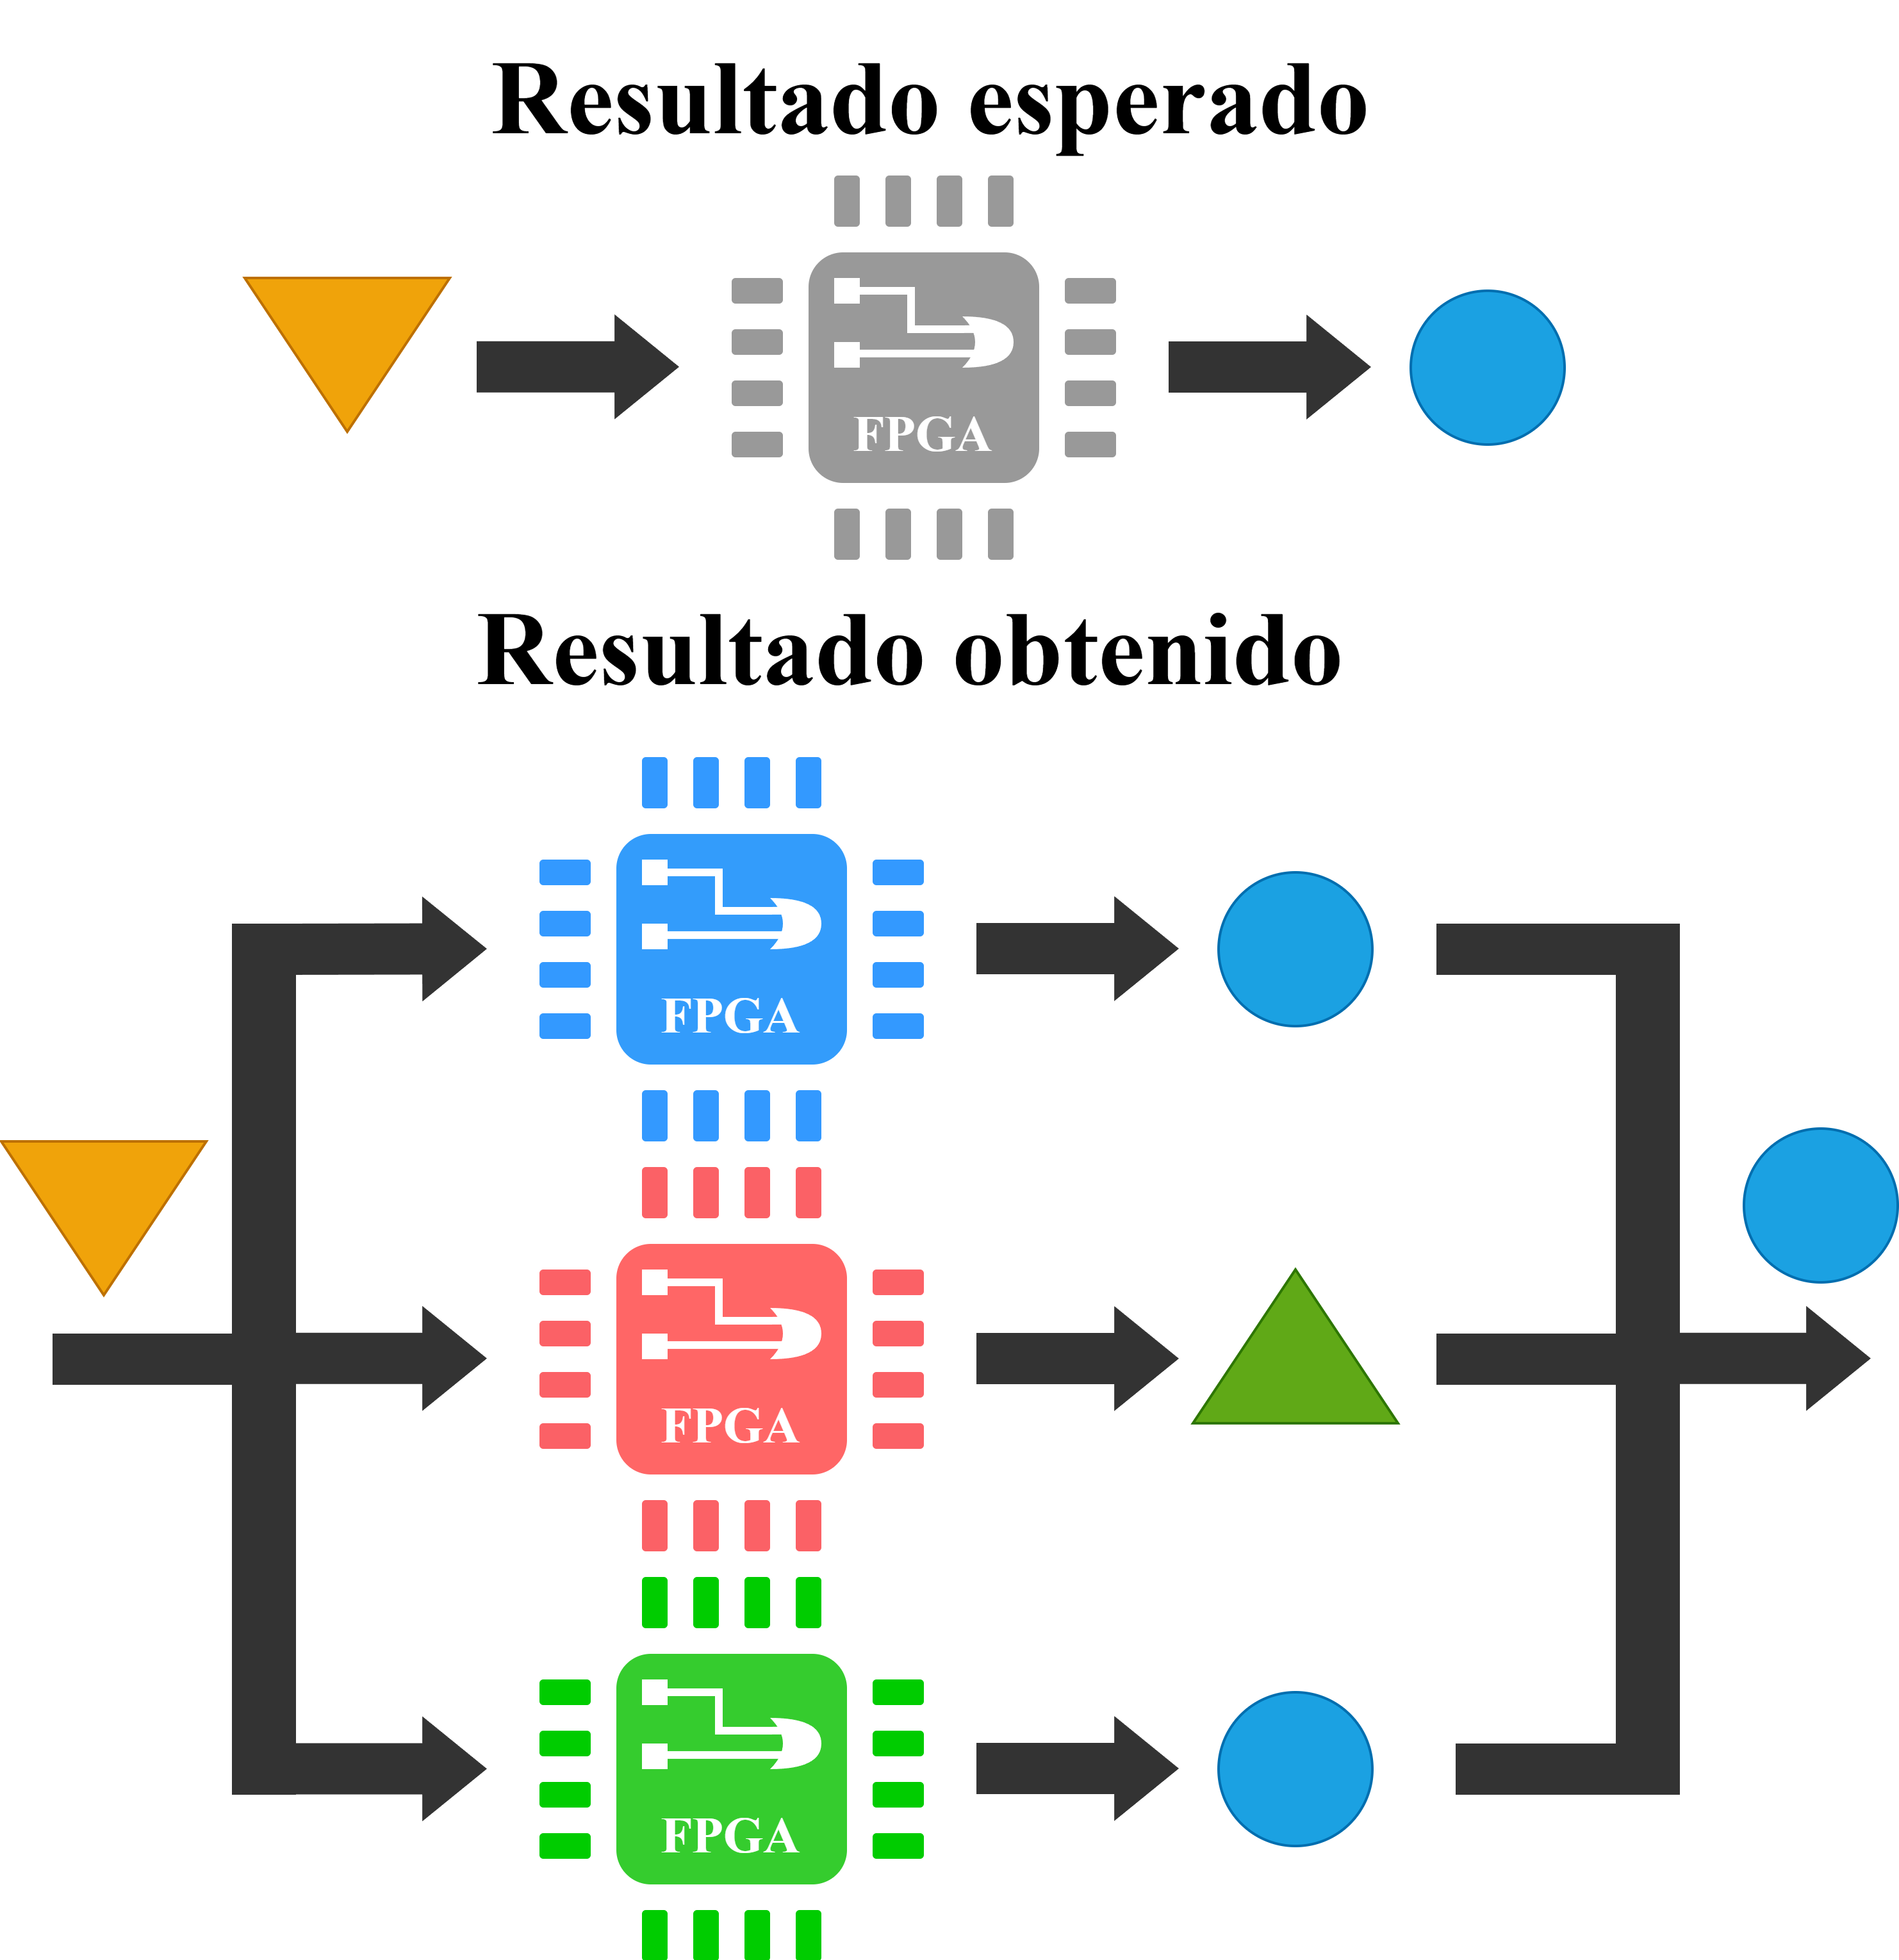
\includegraphics[width=1\textwidth]{Figuras/redundancia.png}
		\centering\caption{Sistema con redundancia 2oo3 y diversidad.}
		\label{fig:redundancia}
	\end{figure}
	
	La tasa de fallas de los sistemas utilizados debe ser lo mas pequeña posible. Existen fallas de causa común asociadas al fabricante de componentes, defectos eléctricos en los materiales, desperfectos en el software replicados en cada uno de los módulos, etc \cite{Paper_30,Paper_32,Paper_42,Paper_47,Paper_77,Paper_83,Paper_84,Paper_118,Paper_122,Paper_124,Paper_125,Paper_127,Paper_131,Paper_132,Paper_136,Paper_138,Paper_140}. Para mitigar las fallas de causa común y robustecer el sistema, se aplica el concepto de diversidad \cite{Paper_53,Paper_125,Paper_131,Paper_132,Paper_140,Paper_171}. En el caso de la Figura \ref{fig:redundancia}, esta diversidad está representada en los módulos de diferentes colores: azul, rojo y verde. De esta forma se busca simbolizar que los tres sistemas cumplen la misma función, pero de manera diferente (distintas plataforas y/o distinto lenguaje de programación o incluso diferente equipo de desarrollo). Los tres módulos tendrán, por lo tanto, tasas de falla distintas. Se asume, además, que los módulos pueden tener fallas simultáneas pero de probabilidad mucho mas baja que la tasa de fallas inherente a cada módulo.
	
	De la investigación realizada surge que el 66\% de las empresas utiliza una redundancia 2oo2 o 2oo3 para alcanzar los niveles de seguridad requeridos \cite{SIEMENS,ALSTOM,HITACHI,THALES,BOMBARDIER,KYOSAN,HIMA,CRRC,CAF,TRANSMASHHOLDING,HYUNDAI,GENERAL,CATERPILLAR,STADLER}. Solo una pequeña porción de las mismas utiliza redundancias 1oo2 \cite{ALSTOM} o 2oo4 \cite{HITACHI}. En consecuencia, se puede afirmar que una redundancia 2oo2 o 2oo3 es representativa de los sistemas analizados y puede utilizarse como esquema de partida para un diseño propio.